\chapter{The Single Skill That Built His \$100M Year Business}

Johnny Anton's interview is not a blackboard lecture, but it does have a clear operating logic. The School of Hard Knocks frame is biographical and commercial: a salesman from a difficult background learns to create revenue, helps scale companies past nine figures, and then tries to explain the habits and systems underneath that result. In these notes, we keep the claims source-conscious. Johnny's stories remain stories, his business claims remain attributed claims, and the equations are compact reconstructions of the loops and mechanisms described in the conversation. This chapter is curated for the LazyEarn track by LazyingArt LLC using Video2Book.

\section{The Portable Skill}

The interview begins by making Johnny a witness. He is introduced as the child of Iraqi immigrants, raised in a poor part of Detroit, homeless for two years, and later involved in scaling multiple businesses to more than nine figures in revenue. That opening does not merely decorate the interview. It tells us why the first claim matters.

The claim is that sales is portable. Markets can crash, crypto can fall, fraud can appear, and a person can still walk into a business with demand and create revenue. In the language of these notes, sales is treated as a revenue-producing skill, not merely as charm or talking.

A compact reconstruction of the opening claim is

\begin{equation}
\text{portable wealth skill}
\quad \approx \quad
\text{ability to create revenue under changing conditions}.
\end{equation}

This is not a formula from a board. It is the first abstraction of the interview. We begin with it because the rest of the conversation asks what sort of inner discipline, feedback system, and business structure can make such a skill durable.

\section{Failure Without Significance}

The first direct question asks what Johnny would tell his younger self. His answer is blunt: fail faster, and do not make failure mean something final about who you are. Notice the order. Before we get to sales scripts, hiring, capital, or product, we get the interpretation of a bad result.

Let \(A_t\) denote an action or attempt at time \(t\), \(R_t\) the result, and \(L_t\) the lesson extracted from the result. The learning loop is

\begin{equation}
A_t \longrightarrow R_t \longrightarrow L_t \longrightarrow A_{t+1}.
\end{equation}

The obstacle is that many people insert an identity judgment between \(R_t\) and \(L_t\). Let \(S_t\) denote the significance load attached to the result. Johnny's point is that the loop accelerates when \(S_t\) is reduced:

\begin{equation}
S_t \downarrow
\quad \Longrightarrow \quad
R_t \text{ becomes usable information}
\quad \Longrightarrow \quad
A_{t+1} \text{ arrives sooner}.
\end{equation}

He motivates this with a claim about startup culture: failing forward intelligently, learning from mistakes, compounding time, and removing the significance of everything. The chapter should not turn that country-level comparison into an external fact without verification. But inside the interview it does a clear job: it makes failure part of a compounding process rather than a verdict.

\subsection{Question \& Answer}

\paragraph{Question.}
Why would failing faster help if failure still costs time, money, and reputation?

\paragraph{Answer.}
Because the cost of failure is not only the external loss. It is also the delay caused by making the result mean too much. The productive loop is

\begin{equation}
\text{attempt}
\rightarrow
\text{result}
\rightarrow
\text{lesson}
\rightarrow
\text{next attempt}.
\end{equation}

The stalled loop is

\begin{equation}
\text{attempt}
\rightarrow
\text{result}
\rightarrow
\text{identity verdict}
\rightarrow
\text{avoidance or delay}.
\end{equation}

Johnny's advice is to protect the first loop. Failure can compound into judgment, or it can compound into information.

\section{The Three Habits And The Feedback Loop}

The interviewer then asks for the habits that made Johnny successful. Johnny gives three. The first is meditation, which he describes as reconditioning the mind. He says he had been meditating consistently for more than six years and first learned the practice at a wrestling camp, where the target was winning a state championship. He then connects meditation to imagination: before something exists in the material world, one has to be able to hold it as a possibility.

His example is Walt Disney. In Johnny's telling, Disney imagined the park before it existed, faced repeated banker refusals, needed a \( \$5 \) million loan, and saw the project later cost \( \$15 \) million. We should keep this as an attributed story. Its function in the argument is to say: a future result must first become thinkable.

The second habit is more operational: take consistent action and document what is working and what is not. Johnny says his sales team uses an end-of-day report. The report asks who was contacted, what happened, what worked, what did not work, and who the salesperson was being behind the words.

The third habit is to pay people who already have the desired results. Johnny's phrase is to cut checks faster and bigger. The idea is not spending for status. It is buying proximity to pattern recognition.

The three habits can be summarized as

\begin{align}
\text{Habit 1} &: \text{make the desired future thinkable},\\
\text{Habit 2} &: \text{act, measure, report, and revise},\\
\text{Habit 3} &: \text{model people with proven patterns}.
\end{align}

The second habit gives the strongest mathematical spine of the chapter. A sales day is not just activity. It is an iteration:

\begin{equation}
\text{Calls}_t
\longrightarrow
\text{Report}_t
\longrightarrow
\text{Adjustment}_t
\longrightarrow
\text{Calls}_{t+1}.
\end{equation}

A useful report has fields:

\begin{equation}
\text{Report}_t =
\{
\text{contacts},
\text{call result},
\text{worked},
\text{did not work},
\text{state/context}
\}.
\end{equation}

That last term is where Johnny slows the discussion down. He is not satisfied with the words alone. He wants to know who the salesperson was being behind the words.

\subsection{Question \& Answer}

\paragraph{Question.}
If two salespeople use the same script, why does one outperform the other?

\paragraph{Answer.}
Because the script is not the whole system. Johnny's answer is that context can matter more than content. The same words can be delivered with different certainty, attention, timing, emotional state, and understanding of the prospect.

A cautious reconstructed model is

\begin{equation}
O =
f(
\text{offer},
\text{prospect},
\text{script},
\text{context},
\text{salesperson state}
),
\end{equation}

where \(O\) is the sales outcome. This is not meant as a measured statistical model. It is a way of preserving the interview's central distinction: visible content does not exhaust the causes of the result.

\subsection{A Worked Update Rule}

Let \(c_t\) be the number of meaningful conversations on day \(t\), \(w_t\) the set of observed behaviors that worked, \(n_t\) the set that did not work, and \(q_t\) a qualitative description of the salesperson's state. Then

\begin{equation}
\text{Report}_t=(c_t,w_t,n_t,q_t).
\end{equation}

The next day's action plan is updated from that report:

\begin{equation}
A_{t+1}=U(A_t,\text{Report}_t),
\end{equation}

where \(U\) means: keep what worked, remove or test what failed, and adjust the state behind the action.

For example, suppose a salesperson makes \(20\) calls. The report says that opening with price created resistance, but opening with the prospect's current constraint created better conversation. The update is

\begin{align}
A_t &: \text{lead with price and offer},\\
\text{Report}_t &: \text{resistance high; diagnosis questions worked},\\
A_{t+1} &: \text{lead with the current constraint, then bridge to the offer}.
\end{align}

This is the lecture's practical mathematics: a disciplined update rule rather than a motivational slogan.

\begin{figure}
\centering
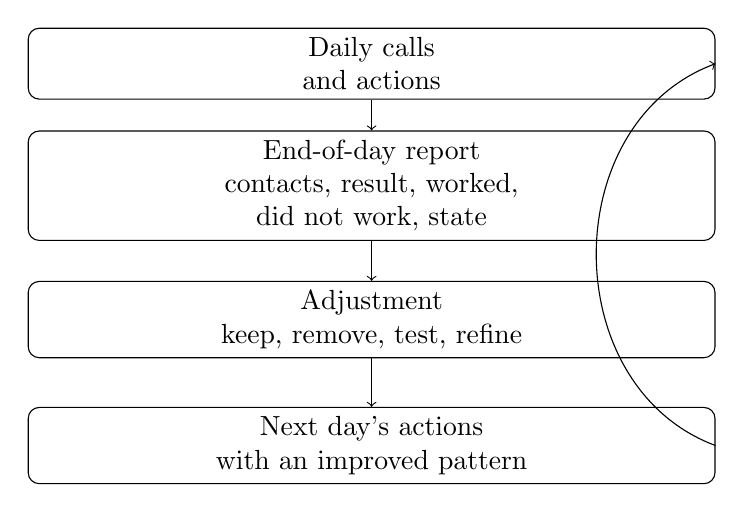
\begin{tikzpicture}
\node[draw, rounded corners, text width=0.70\linewidth, align=center] (calls) at (0,0) {Daily calls\\and actions};
\node[draw, rounded corners, text width=0.70\linewidth, align=center] (report) at (0,-1.55) {End-of-day report\\contacts, result, worked,\\did not work, state};
\node[draw, rounded corners, text width=0.70\linewidth, align=center] (adjust) at (0,-3.25) {Adjustment\\keep, remove, test, refine};
\node[draw, rounded corners, text width=0.70\linewidth, align=center] (next) at (0,-4.85) {Next day's actions\\with an improved pattern};

\draw[->] (calls) -- (report);
\draw[->] (report) -- (adjust);
\draw[->] (adjust) -- (next);
\draw[->] (next.east) .. controls (2.35,-4.1) and (2.35,-0.75) .. (calls.east);
\end{tikzpicture}
\caption{A transcript-grounded reconstruction of Johnny's feedback loop. No validated board diagram was available for this lecture.}
\end{figure}

\section{Pattern Recognition And The Ownership Trap}

Johnny's third habit is pattern recognition by proximity. Find people with the desired result, pay them, watch them, and model what they do. The local model is stimulus and response:

\begin{equation}
S \longrightarrow R.
\end{equation}

Here \(S\) might be a question, a sales frame, a pricing move, or a business action. \(R\) is the prospect's or market's response. Pattern recognition is the ability to see which stimuli tend to produce which responses in which contexts.

\begin{definition}
Pattern recognition, in these notes, means the practiced ability to observe repeated stimulus-response structures and to model people who already produce the desired result.
\end{definition}

Johnny uses wrestling, school, and sales as examples. He says he reached a state championship after only two years of wrestling and performed well academically by studying what had to be done in the moment-to-moment phenomenon. The mechanism is not magic. It is observation, imitation, correction, and repetition.

Then the interview turns. The next question asks what advice Johnny would give himself when starting his first business. His answer is the reversal: ego is not your friend. Because he had helped a company move from high eight figures toward multiple nine figures, he thought running his own company would be easy. His boss Paul challenged him. In a \(100\%\) commission sales role earning about half a million dollars, Johnny did not have to carry marketing, delivery risk, hiring, operations, or finance.

The missing system can be written as

\begin{equation}
\text{Business ownership}
=
\text{sales}
+
\text{marketing}
+
\text{delivery}
+
\text{hiring}
+
\text{operations}
+
\text{finance}
+
\text{risk}.
\end{equation}

A person can be excellent at one term in this sum and still underestimate the whole. That is the point of Paul's warning. Sales mastery creates revenue, but ownership means carrying the entire coupled system.

\begin{remark}
The anecdote should not be reduced to humility in the abstract. Its commercial mechanism is precise: commission sales can hide the full risk-bearing structure of a business. Ownership exposes the missing terms.
\end{remark}

Johnny ties his arrogance to an old identity and a desire to prove himself. We keep that as anecdote. The mechanism that follows is more general: if the desired result already exists somewhere, ego is expensive when it prevents modeling it.

\section{Scaling Beyond Sales}

The next question moves from the first business to scale: what takes a business from seven to eight figures, and from eight to nine? Johnny cites Ryan Breslow as a model and says the answer comes down to fundraising and recruiting. He then expands the chain: cash is needed to scale, cash and hiring depend on leadership, leadership depends on vision, talent requires compensation, and compensation requires a strong product.

The chain is

\begin{equation}
\text{Product}
\longrightarrow
\text{Vision and leadership}
\longrightarrow
\text{Fundraising and recruiting}
\longrightarrow
\text{Talent}
\longrightarrow
\text{Scale}.
\end{equation}

This is the section where the interview leaves the individual closer and moves toward enterprise construction. Sales remains essential, but no longer sufficient. A business that aims at nine figures must attract leadership, capital, and talent.

\begin{figure}
\centering
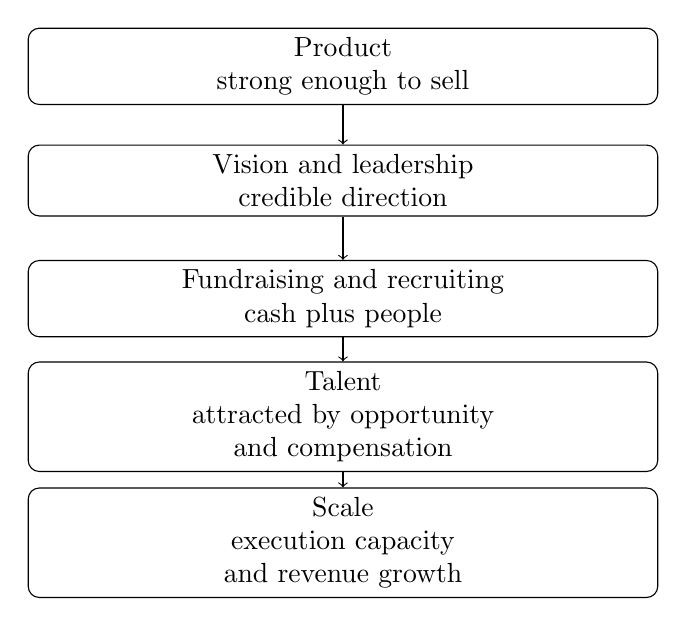
\begin{tikzpicture}
\node[draw, rounded corners, text width=0.64\linewidth, align=center] (product) at (0,0) {Product\\strong enough to sell};
\node[draw, rounded corners, text width=0.64\linewidth, align=center] (vision) at (0,-1.45) {Vision and leadership\\credible direction};
\node[draw, rounded corners, text width=0.64\linewidth, align=center] (fund) at (0,-2.95) {Fundraising and recruiting\\cash plus people};
\node[draw, rounded corners, text width=0.64\linewidth, align=center] (talent) at (0,-4.45) {Talent\\attracted by opportunity\\and compensation};
\node[draw, rounded corners, text width=0.64\linewidth, align=center] (scale) at (0,-6.05) {Scale\\execution capacity\\and revenue growth};

\draw[->] (product) -- (vision);
\draw[->] (vision) -- (fund);
\draw[->] (fund) -- (talent);
\draw[->] (talent) -- (scale);
\end{tikzpicture}
\caption{Johnny's scale chain, reconstructed from the transcript for pocket-size layout.}
\end{figure}

The transcript around this portion contains a long corrupted stretch of repeated ``yeah'' before returning to banking, private equity, and talent. We should not overbuild from the corrupted segment. The reliable through-line is talent: top firms and startups compete for it, and talent requires both compensation and a product worth joining.

\section{Starting From Zero}

The interviewer then resets the game: suppose the bank account is zero. What is the first step? Johnny begins at the bottom. Sell the most expensive thing available until rent, food, and shelter are covered. Once basic survival is handled, the next move is to use skills and connections to create value.

The rebuild sequence is

\begin{equation}
\begin{aligned}
&\text{high-ticket selling}
\rightarrow
\text{food and shelter}
\rightarrow
\text{free value}
\rightarrow
\text{testimonials and case studies}\\
&\rightarrow
\text{anchor client}
\rightarrow
\text{adjacent prospects}
\rightarrow
\text{high-value, low-risk package}
\rightarrow
\text{sales team and lead sources}.
\end{aligned}
\end{equation}

This is one of the interview's clearest operating models. It says: first survive, then create proof, then distribute the proof.

\begin{enumerate}
\item Sell a high-ticket offer to restore immediate cash.
\item Use skills and connections to add value for free.
\item Convert free value into testimonials, case studies, and an anchor client.
\item Use the anchor client to approach competitors, adjacent niches, and first-degree connections.
\item Package the offer with high value and low client risk.
\item Build a sales team and expand lead sources.
\end{enumerate}

The mechanism is proof before scale. The anchor client is not just revenue; it is evidence. Evidence lowers the resistance of the next sale.

\begin{figure}
\centering
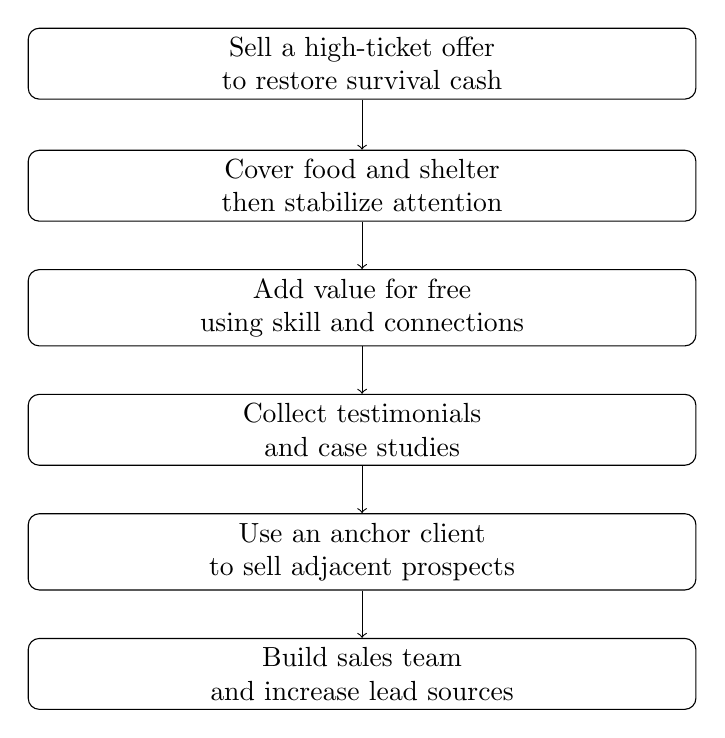
\begin{tikzpicture}
\node[draw, rounded corners, text width=0.68\linewidth, align=center] (a) at (0,0) {Sell a high-ticket offer\\to restore survival cash};
\node[draw, rounded corners, text width=0.68\linewidth, align=center] (b) at (0,-1.55) {Cover food and shelter\\then stabilize attention};
\node[draw, rounded corners, text width=0.68\linewidth, align=center] (c) at (0,-3.10) {Add value for free\\using skill and connections};
\node[draw, rounded corners, text width=0.68\linewidth, align=center] (d) at (0,-4.65) {Collect testimonials\\and case studies};
\node[draw, rounded corners, text width=0.68\linewidth, align=center] (e) at (0,-6.20) {Use an anchor client\\to sell adjacent prospects};
\node[draw, rounded corners, text width=0.68\linewidth, align=center] (f) at (0,-7.75) {Build sales team\\and increase lead sources};

\draw[->] (a) -- (b);
\draw[->] (b) -- (c);
\draw[->] (c) -- (d);
\draw[->] (d) -- (e);
\draw[->] (e) -- (f);
\end{tikzpicture}
\caption{The starting-from-zero ladder implied by Johnny's answer.}
\end{figure}

\section{Sales As Transfer Of Certainty}

The final substantive question asks how Johnny turns a no into a yes. He reframes the question. The deeper problem is not overcoming objections after they appear. It is understanding the buyer well enough that the presentation is already built around the buyer's real situation.

He divides buyer understanding into demographics and psychographics. Demographics identify who the prospect is in observable terms: age, background, origin, family context, life situation. Psychographics identify what moves the person: interests, desires, fears, behaviors, psychology, and decision patterns.

\begin{table}
\centering
\begin{tabular}{|p{0.42\linewidth}|p{0.42\linewidth}|}
\hline
\textbf{Demographics} & \textbf{Psychographics} \\
\hline
Age, background, origin, family context, life situation & Interests, desires, behavior, fears, psychology, decision pattern \\
\hline
Who the person is in observable terms & How the person interprets problems and makes choices \\
\hline
\end{tabular}
\caption{A transcript-grounded reconstruction of Johnny's buyer-understanding split.}
\end{table}

Johnny's definition of sales is a transfer of certainty. A product or service must bridge the buyer's current situation to the buyer's desired situation:

\begin{equation}
\text{current situation}
\xrightarrow{\text{product/service plus certainty}}
\text{desired situation}.
\end{equation}

\subsection{Question \& Answer}

\paragraph{Question.}
How do we turn a no into a yes?

\paragraph{Answer.}
In Johnny's framing, we do not start with the objection. We start with the person. We ask where the buyer is, where the buyer wants to go, and what the buyer cares about. The offer is not forced as our agenda. It is presented as the bridge between the buyer's current state and desired state.

The compact model is

\begin{equation}
\text{Sales}
=
\text{diagnosis}
+
\text{certainty}
+
\text{credible bridge}.
\end{equation}

Diagnosis comes from understanding the buyer. Certainty comes from the salesperson's own psychology and command of the offer. The credible bridge is the product or service positioned against the buyer's stated problem.

\section{Summary}

The interview begins with Johnny as evidence that sales can be a portable wealth skill. It then moves step by step: fail faster, reduce the significance of failure, use meditation to reshape what seems possible, act consistently, report results, model proven patterns, avoid the ego trap of mistaking sales skill for full ownership, recruit talent for scale, rebuild from zero through proof, and sell by diagnosing the buyer's current and desired states.

The central loop is

\begin{equation}
A_t \longrightarrow R_t \longrightarrow L_t \longrightarrow A_{t+1}.
\end{equation}

The strongest operating mechanism is the feedback rule

\begin{equation}
\text{action}
\longrightarrow
\text{measurement}
\longrightarrow
\text{adjustment}
\longrightarrow
\text{improved action}.
\end{equation}

And the final sales mechanism is the bridge:

\begin{equation}
\text{current situation}
\longrightarrow
\text{desired situation}.
\end{equation}

There are no validated board screenshots or visible equations for this lecture, so the diagrams are reconstructions rather than visual evidence. The source-conscious reading is the important discipline: anecdote remains anecdote, claim remains attributed claim, and mechanism is extracted from the order in which the interview unfolds.